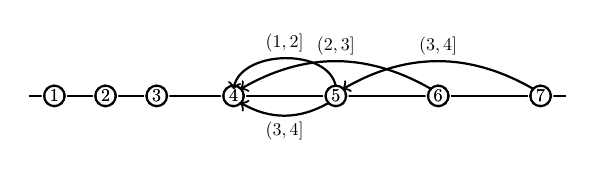
\begin{tikzpicture}[thick,scale=0.65, every node/.style={scale=0.65}]
\draw (0,0) -- (10.5,0);
\foreach \x [count=\xi] in {0.5, 1.5, 2.5, 4, 6, 8, 10} {
    \fill[white] (\x,0) circle (0.25);
    \ifthenelse{\xi = 4}
    {\draw[dotted] (\x,0) circle (0.2) node {$\xi$};}
    {\draw (\x,0) circle (0.2) node {$\xi$};}
}
\def\offset{0.13}
\draw [->] (10-\offset,0+\offset) to [out=150,in=30] node[midway, above] {$(3,4]$} (6+\offset,0+\offset);
\draw [->] (8-\offset,0+\offset) to [out=150,in=30] node[midway, above] {$(2,3]$} (4+\offset,0+\offset);
\draw [->] (6,0+\offset+.05) to [out=100,in=80] node[midway, above] {$(1,2]$} (4,0+\offset);
\draw [->] (6-\offset,0-\offset) to [out=-150,in=-30] node[midway, below] {$(3,4]$} (4+\offset,0-\offset);
\end{tikzpicture}